Dieses Kapitel bietet einen Überblick über einige p2p-Netzwerke und evaluiert diese anhand gestellter Anforderungen. Diese Evaluierung beeinflußt die Entscheidung für ein Overlay-Netzwerk, auf das schließlich, das in dieser Arbeit zu entwickelnde, generische Publish/Subscribe-System gesetzt wird. Die Evaluierung bedient sich zahlreicher Arbeiten, die sich alleine dem Vergleich dieser Netzwerke widmen \cite{Lua2005Survey, Goetz2005, Li2004Comparing, Darlagiannis2006Peertopeer, Castro2002Secure, Bo2003PeertoPeer} und geht auch auf ihre Nutzbarkeit als Basis für \emph{Application level multicast} sprich ein Publish/Subscribe-System ein \cite{Hosseini2007Survey, Fahmy2007, Castro2003Evaluation, Ratnasamy2001}.

Zuvor müssen jedoch die eigenen Anforderungen an solche Systeme identifiziert werden. Zu den offensichtlichen Anforderungen wie beispielsweise \emph{Skalierbarkeit} gesellen sich jedoch auch spezielle Anforderungen aus Spielsicht hinzu. Diese sind beispielsweise das Vorhandensein eines Masterservers oder das Übertragen von Applikationswissen auf das Netzwerk um damit dessen Entscheidungen bezüglich Nachbarschaften oder Versand von Nachrichten (Routing) zu beeinflussen.

\section{Anforderungen}

\paragraph{Geringe Latenz} Schnelle Reaktionszeiten und Nachrichtenübermittlung sind bei \ac{mmog} unverzichtbar. Ebenfalls müssen größere Nachrichten (beispielsweise Update der Welt) schnell übertragen werden damit der Spielfluss nicht behindert wird. Dies lässt sich anhand der Anzahl der Hops beim Nachrichtenversand messen.

\paragraph{Skalierbar} Selbst bei einer großen Anzahl an Knoten soll das Netz nicht kollabieren. Hierbei ist es auch wichtig, dass Knoten nicht unbedingt lange im Spiel sein müssen. Zwar kann davon ausgegangen werden, dass ein durchschnittlicher Spieler längere Zeit im Spiel verbringt, aber durch Netzausfälle oder sonstigen Unbill kann dies stark variieren. Insofern ist es wichtig wie sich die Netzwerke bei großen Fluktationen verhalten \cite{Li2004Comparing}.

\paragraph{Fehlertoleranz bei Knotenausfall} Fallen Knoten aus, muss sich das Netz ohne großen Kommunikationsaufwand selbst reparieren. Ebenfalls mögliche Netzwerkpartitionierungen sind in dieser Arbeit jedoch kein Hindernis, denn der Hauptserver kann über eine gesonderte Verbindung immer erreicht werden. Damit kann das Netz wieder verbunden werden.\\
Interessant hierbei ist auch die eingebaute Redundanz einiger Systeme, die Daten auf mehrere Knoten verteilen. Wie sich dies im Vergleich von statischen Daten zu sich häufig verändernden Objekten der Spielewelt verhält ist zu untersuchen. 

\paragraph{Kommunikation über das Netzwerk} Das Netzwerk soll nicht nur das schnelle Auffinden von Peers ermöglichen, sondern auch einen Transport der Nachricht (Routing) durch das Netzwerk selbst bereitstellen. Die Alternative Direktverbindungen soll nur genutzt werden, wenn eine Datenübertragung im Netzwerk nicht performant genug ist, weil z.B. die Bandbreite der zwischengeschalteten Peers zu gering ist.

\paragraph{Bestimmung der Nachbarschaft} Eine dynamische Bestimmung der Nachbarschaftsgröße kann von Vorteil sein. So könnten Knoten mit mehr Bandbreite (bzw. entsprechenden anderen Metriken) mehr direkte Verbindungen halten als Knoten mit geringer Bandbreite (oder geringer Spieldauer).

\paragraph{Eingriff in Routingentscheidungen} Applikationswissen hilft auch beim Eingriff in das Routing des Netzes. So können Knoten bevorzugt zur Weiterleitung einer Nachricht ausgewählt werden. Diese Knoten zeichnen sich beispielsweise durch eine große Bandbreite oder spezielle Applikationsmetriken\footnote{Bsp: Spieler befindet sich in der selben Stadt} aus.

\paragraph{Verfügbarkeit als C/C++-Bibliothek} Da der Prototyp dieser Arbeit sowie das Umfeld in C++ entwickelt wird, gibt es damit eine weitere Anforderung an das Netzwerk: Die Verfügbarkeit als C/C++-Bibliothek.\\
Damit ist das Netzwerk einfach aus bestehendem Code nutzbar ohne dass kostenintensive Brücken zwischen beispielsweise Java und C++ geschlagen werden müssen. Da zudem betriebssystemübergreifend\footnote{In unserem Fall auf Windows und Linux} entwickelt und getestet wird, ist außerdem ein zur Verfügung stehender Quellcode vorteilhaft. Nur dadurch ist es möglich eventuellen betriebsystembezogenen Netzwerk- oder Threadcode auf  Boost\footnote{Zahlreiche Bibliotheken für C++: http://www.boost.org} zu portieren um somit eine betriebsystemübergreifende Benutzung zu ermöglichen.

\paragraph{Unterbau eines Publish/Subscribe-Systems} Das Overlay-Netzwerk muss so gestaltet sein, dass es dem Anwendungsfall \emph{Application level multicast} genügt und dessen besondere Anforderungen (auch von Spielseite)\footnote{siehe Kapitel \ref{chap:evaluation_pubsub}} her unterstützt.

Anhand dieser Anforderungen sind unstrukturierte Netzwerke nicht als Netzwerksystem für dieser Arbeit geeignet. Eine Suche, bzw. Datenübertragung durch Flooding widerspricht klar der Anforderung nach geringer Latenz. Ebenso sind diese Netzwerke auf eine Übertragung via Direktverbindung ausgelegt.

\cite{Dabek2003Towards} stellt eine generische \ac{api} für \ac{kbr} Systeme vor, wie es viele der strukturierten Netzwerke anbieten vor und zeigt wie darauf aufbauen verschiedene Systeme wie \ac{dht}, \ac{dolr} und \ac{cast}\footnote{entspricht Application level multicast} implementiert werden können. Ebenfalls wird gezeigt wie einige bekannte Systeme (CAN, Chord, Pastry und Tapestry) diese die Anforderungen erfüllen.\\
Daraus ergibt sich eine weitere spezielle Anforderung an das Overlay-Netzwerk:

\paragraph{Anpassbarkeit an generische \ac{api}} Lässt sich das Netzwerk der genersischen \ac{api} anpassen, gewinnt das an Flexibiliät, da die Netzwerkschicht ohne große Änderungen an den restlichen Systemschichten ausgetauscht und verändert werden kann.

\section{generic API}
\label{chap:evaluation_p2p:generic_api}
\cite{Dabek2003Towards} %towards

\lstinputlisting[caption={Upcalls der generischen API}, label=code:towards_upcall]{listings/towards_upcall.cpp}



\section{Evaluation}
In diesem Kapitel werden die vier bekannten Systeme Chord \cite{Stoica2003}, Pastry \cite{Rowstron2001}, Tapestry \cite{Zhao2001Tapestry,Zhao2004Tapestry} und CAN \cite{Ratnasamy2001Scalable} miteinander verglichen. Die ersten drei sind in ihrem Aufbau ähnlich (Schlüsselraum wird auf einen Ring verteilt) und unterscheiden sich in der Art des Routings. CAN hingegeen bildet den Schlüsselraum auf ein d-dimensionalen kartesisches Koordinatensystem ab. Alle vier Systeme sind laut \cite{Dabek2003Towards} im Hinblick auf die generische \ac{api} nutzbar.

Zur Entscheidungsfindung werden die Netzwerke anhand folgender Gesichtspunkt verglichen:
\begin{itemize}
\item Aufbau und Struktur
\item Routing
\item Nachbarschaft
\item Eintritt und Austritt (Fehlerfall) von Knoten
\item Nutzbarkeit als Basis für \ac{cast}
\end{itemize}

\subsection{Aufbau und Struktur}
\paragraph{Chord}
Chord \cite{Stoica2003} legt die l-bit wertigen Schlüssel (meist Zahlen im Bereich $[0,2^l-1]$) auf einem eindimensionalen Ring modulo $2^l$ im Uhrzeigersinn an. Jedem Knoten und jedem Datum ist ein eindeutiger Schlüssel zugewiesen, diese sind \emph{ID} und \emph{key} benannt. Ein Datum $X$ ist dem Knoten zugewiesen, dessen ID größer gleich dem key ist. Dieser Knoten wird Nachfolger von X, \emph{SUCC(X)}, genannt. Analog dazu gibt es auch einen Vorgänger von X, \emph{PRED(X)}.

Damit ist ein Knoten für alle Daten zuständig, die - bildlich gesehen - im Ring gegen den Uhrzeigersinn vor ihm liegen. In Abbildung \ref{fig:chord_key_space} a ist dies bildlich für sechs Knoten und fünf Datenpunkten bei $l=6$ gezeigt. Knoten 14 (N14) ist für das Datum mit Schlüssel 10 (K10) zuständig. Knoten 32 ist für K16 und K25. K51 ist bei N51 zu finden. Aufgrund der Ringstruktur ist N1 für K55 zuständig.

\begin{figure}[htb]
\centering
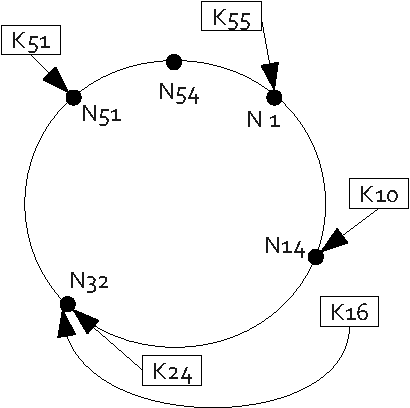
\includegraphics{grafics/chord_key_space.pdf}
\caption{(a) Schlüsselraum ($l=6$) für Chord mit sechs Knoten ($Nx$) und fünf Daten ($Kx$). Die gestrichelten Pfeile stellen die Einträge der Fingertabelle für Knoten $N1$ dar (b).}
\label{fig:chord_key_space}
\end{figure}


\paragraph{Pastry / Tapestry}
Pastry \cite{Rowstron2001} und Tapestry \cite{Zhao2001Tapestry,Zhao2004Tapestry} sind sich sehr änlich, da beiden auf Plaxtons Arbeit \cite{Plaxton1997Accessing} aufbauen. Auf Unterschiede wird explizit hingewiesen.

Pastry besitzt ebenfalls einen l-bit wertigen Schlüsselraum, dabei werden Schlüssel als Zahlen zur Basis $2^b$ dargestellt\footnote{l meist 128; b meist 4}, wobei die Wahl von $b$ einen Einfluss auf das Routing hat. Ein Datum ist dem Knoten zugewiesen, dessen ID am nähsten zum Schlüsselwert des Datums liegt.  Abbildung \ref{fig:pastry_key_space} zeigt dies beispielhaft für sechs Knoten und fünf Datensätzen. Im Unterschied zu Chord ist hier Knoten $N14$ für $K16$ und Knoten $N54$ für $K55$ zuständig.\\
\missing{Noch nicht so sehr schön beschrieben!}

Tapestry erzeugt automatische Redundanz, da hier die Daten auf mehrere Knoten verteilt werden.

\begin{figure}[htb]
\centering
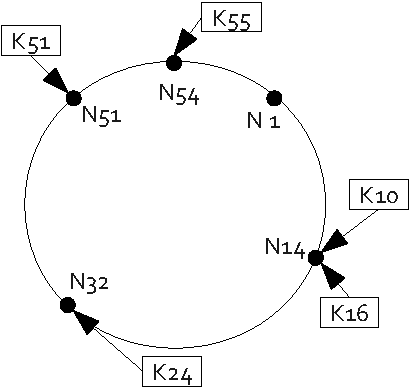
\includegraphics{grafics/pastry_key_space.pdf}
\caption{Schlüsselraum ($l=4$) für Pastry mit sechs Knoten ($Nx$) und fünf Daten ($Kx$).}
\label{fig:pastry_key_space}
\end{figure}


\paragraph{CAN}

\begin{figure}[htb]
\centering
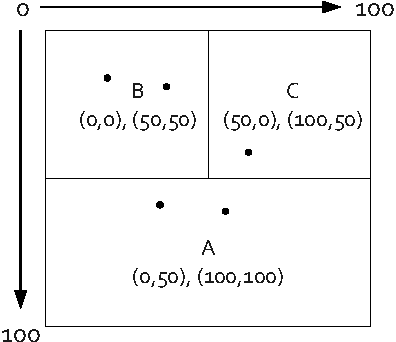
\includegraphics{grafics/can_key_space.pdf}
\caption{2-dimensionaler Schlüsselraum (0,0) bis (100,100) für CAN mit drei Knoten (A, B, C) und fünf Daten (schwarze Punkte).}
\label{fig:can_key_space}
\end{figure}


\subsection{Routing}
\paragraph{Chord}
Bei Chord besitzt jeder Knoten eine Verbindung zu seinem direkten Vorgänger und seinem direkten Nachfolger. Eine Nachricht wird an den Nachfolger geschickt, bis sie zum zuständigen Knoten gelangt. Bei einer \emph{LOOKUP(x)}-Nachricht\footnote{Suche für key x Knoten N, so dass gilt: $N = SUCC(x)$.} prüft jeder involvierte Knoten A, ob sein Nachfolger für den Schlüssel zuständig ist, d.h. $ID_A < x \le SUCC(A)$. Ist dies der Fall, so sendet Knoten A die Anwort SUCC(A) rückwärts den Pfad der Nachricht zurück. Bei normalem Nachrichtenaustausch wird die Nachricht an den entsprechenden Knoten weitergeleitet.

Da dies eine sehr ineffizientes  Routing darstellt, pflegt jeder Knoten eine sogenannte \emph{finger table}. Die maximal $l$ Einträge in dieser Tabelle zeigen auf andere Knoten im Ring, so dass der Eintrag in Zeile $i$ von Knoten $n$ denjenigen Knoten enthält der $n$ mit mindestens $2^{i-1}$ folgt.\\
Abbildung \ref{fig:chord_key_space} b stellt die Fingertabelle von Knoten $N1$ dar. Die ersten Einträge SUCC(2), SUCC(3) und SUCC(5) verweisen auf Knoten $N5$. Der dritte Eintrag verweist auf $SUCC(9) = N14$. Analog dazu ergeben sich die restlichen Einträge.

Über diese Fingertabelle können Nachrichten eine weiter Strecke auf dem Ring überbrücken und die Routingzeit wird stark verkürzt. Da die IDs in der Tabelle exponential zur Basis zwei ansteigen, halbiert sich die Distanz zum Ziel. Damit hat das Routing eine Komplexität von $O(log N)$.

\paragraph{Pastry / Tapestry}
Jeder Knoten verwaltet neben dem ihm zugeteilten Daten drei Strukturen die dem Routing dienen. Diese sind das \emph{leaf set} mit Einträgen zu Knoten die im Schlüsselraum naheliegen, das \emph{neighborhood set} mit Einträgen zu Knoten die aus Netzwerksicht nahe liegen und die Routingtabelle.

\begin{figure}[htb]
\centering
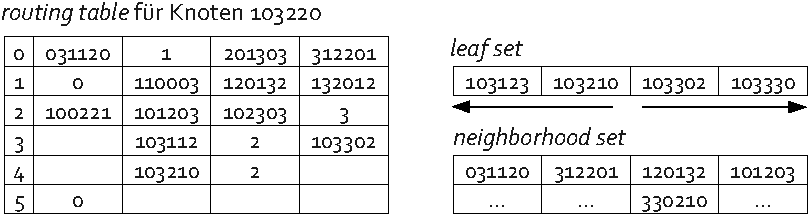
\includegraphics{grafics/pastry_routing_table.pdf}
\caption{Routing table, leaf set und neighborhood set (nach \cite{Goetz2005}) des Knoten 103220 für $l=12, b=2$. Einträge in Zeile $i$ haben einen Präfix der Länge $i$ mit dem Knoten $103220$ gemein.}
\label{fig:pastry_routing_table}
\end{figure}

Die Routingtabelle besteht aus $\frac{l}{b}$ Reihen mit je $2^b -1$ Einträgen. Abbildung \ref{fig:pastry_routing_table} zeigt dies beispielhaft für Knoten $103220$ mit $l=12, b=2$. Einträge in Zeile $i$ haben einen Präfix der Länge $i$ mit dem Knoten $103220$ gemein. Die Übereinstimmungen sind in der Abbildung fett hervorgehoben. Ist kein passender Knoten bekannt, wird das entsprechende Feld nicht ausgefüllt. Damit hat die Routingtabelle Ähnlichkeiten zur Fingertabelle bei Chord. Ein Knoten hat ungenaues Wissen über entfernte Knoten. Der Detailgrad an Routinginformationen erhöht sich pro Zeile in der Routingtabelle. Wenn im System nur sehr wenig Knoten vorhanden sind, dann sind die letzten Reihen der Routingtabelle ebenfalls nur spärlich belegt. Im Durchschnitt sind bei $n$ Knoten im System nur $log_{2^b} n$ Einträge belegt.\\
Bei der Belegung der Routingtabelle werden bei gleichem Präfix diejenigen Knoten gewählt, die aus Netzwerksicht näher sind.

Pastry genügt den Anforderungen der generischen \ac{api} und ruft in jedem Routingschritt die upcall-Funktion route\_message auf. Durch diese kann gezielt in Routingentscheidungen eingegriffen werden und durch Applikationswissen besser gelegene Knoten als Routinghinweis genutzt werden.

\subsection{Nachbarschaft}
\paragraph{Chord}
Die Nachbarschaft ist bei Chord begrenzt. Jeder Knoten hat eine Verbindung zu seinem Vorgänger sowie Nachfolger auf dem Ring und hält Einträge in der Fingertabelle vor. In die Routingentscheidungen kann somit nicht direkt eingegriffen werden.

\missing{routing-upcalls? Eingriff in Entscheidungen?}

\paragraph{Pastry / Tapestry}
Das neigborhood set (siehe Abbildung \ref{fig:pastry_routing_table}) enthält die $|m|$ nähsten Knoten aus Netzwerksicht. Obwohl es im Routing keine Rolle spielt kann es dazu genutzt werden in späteren Entscheidungen geeignete Knoten zu finden.\\
Da die Größe des leaf set ebenfalls wählbar ist, können hier ebenfalls vermehrt nahe Knoten platziert werden.

\paragraph{CAN}
Da nur beim Eintritt eines Knotens in das Netzwerk auf die Nähe aus Netzwerksicht geachtet werden kann, sind die genau $2d$ Nachbarn eines Knotens nicht unbedingt nahe.

\subsection{Eintritt und Austritt (Fehlerfall) von Knoten}
\paragraph{Chord}
Bei Chord kann die ID für einen neuen Knoten $n$ frei gewählt werden, es muss lediglich ein Knoten $b$ im System bekannt sein. n routet eine LOOKUP(n)-Nachricht via b und erfährt somit seinen Nachfolger auf dem Ring. In gleicher Weise vervollständigt $n$ seine Fingertabelle. Weiterhin teilt $n$ seinem Nachfolger mit, dass $n$ sein neuer Vorgänger ist.

Zur Stabilisierung und Vervollständigung der Routinginformationen arbeitet jeder Knoten im Ring periodisch die Funktion \emph{stabilize} ab. Jeder Knoten $a$ fragt seinen Nachfolger $n$ nach dessen Vorgänger $s$. Wenn $a != s$, so ist Knoten $s$ neu in den Ring eingetreten. $a$ informiert den neuen Knoten $s$, dass er sein Vorgänger ist und ändert selbst den eigenen Nachfolger auf $s$ ab. $a$ kennt nun den Bereich seiner Zuständigkeit $[ID_a, PRED(a)[$ und kopiert diese Daten von seinem Nachfolger und weißt diesen auf die Zuständigkeitsänderung hin.\\
Die Aktualisierung der Fingertabelle \emph{fix\_fingers} wird ebenfalls auf jedem Knoten periodisch angestoßen. Für einen zufällig gewählten Eintrag wird überprüft ob dieser noch aktuell ist.

Die Verzögerte Aktualisierung hat keinen großen Einfluß auf die Korrektheit oder Geschwindigkeit des Routings, da Nachrichten an $a$ über die Nachfolger- beziehungsweise Vorgängerverbindungen der Knoten um $a$ weitergeleitet werden und somit lediglich ein weiterer Knoten involviert ist.\\
Bei einer LOOKUP(n)-Nachricht gibt der Vorgänger von n den jeweils richtigen Knoten zurück oder leitet diese Nachricht noch einmal an seinen Nachfolger weiter. Bei einer normalen Nachricht, die zum Nachfolger geroutet werden würde, kann dieser feststellen, dass er nicht mehr für das Datum zuständig ist und die Nachricht an seinen Vorgänger weiterleiten beziehungsweise selbst antworten, wenn die Daten noch nicht umkopiert sind. 

Dies bedeutet allerdings, dass der neue Knoten $n$ erst später von seinem Vorgänger erfährt und damit auch erst spät alle ihm zugeteilten Daten kennt und zu sich übertragen kann. Hier stellt sich nun die Frage, warum $n$ nicht beim Eintritt seinen Nachfolger $p$ nach dessen altem Vorgänger fragt und somit die Zuständigkeit der Daten gleich beim Eintritt klärt? Eine mögliche Antwort ist, dass dadurch viel Overhead durch das Umkopieren von Daten entstehen würden, ohne dass dadurch das Routing bzw. Auffinden der Daten merklich verbessert würde. Im Falle von häufigen Eintritt und Austritt von Knoten würde das Netz lahmgelegt.

Abbildung \ref{fig:chord_new_node} verdeutlich den Neueintritt von Knoten $N20$. Die Änderungen sind in grün dargestellt. $N1$ passt seine Fingertabelle an und $N20$ ist für $K16$ zuständig.

\begin{figure}[htb]
\centering
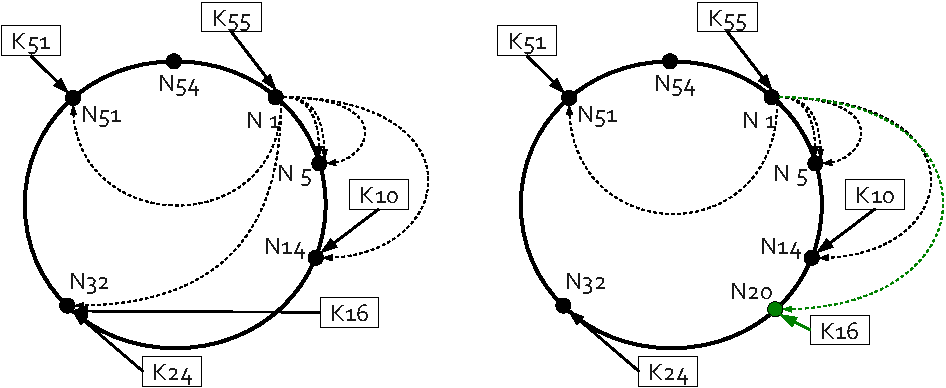
\includegraphics{grafics/chord_new_node.pdf}
\caption{Schlüsselraum von Abbildung \ref{fig:chord_key_space} nach Ankunft von Knoten $N20$. Die Zuständigkeit für $K16$ sowie die Fingertabelle von $N1$ (gestrichelte Linien) wurden angepasst.}
\label{fig:chord_new_node}
\end{figure}

Der Ausfall von Knoten wird über \emph{timeouts} ermittelt. Tritt ein timeout auf, so wird die Nachricht einfach an den besten bekannten Vorgänger des ausgefallenen Knotens weitergeleitet. Im schlimmsten Falle ist dies der Nachfolger des sendenden Knotens. Daraus wird ersichtlch, dass ein valider Nachfolger notwendig ist. Somit hält jeder Knoten eine Liste von möglichen Nachfolgern vor, die während \emph{stabilize} erstellt werden kann. Für fehlerhafte Knoten in der Fingertabelle kann \emph{fix\_fingers} explizit aufgerufen werden.

Knotenaufall bedeutet nicht nur einen Ausfall des Knotens, sondern bedingt, dass die dort gespeicherten Daten nicht mehr erreichbar sind. Da bei Chord immer SUCC(key) für das jeweilige Datum zuständig ist, empfiehlt es sich auf Applikationsebene die Daten auf Knoten $n$ und $SUCC(n)$ zu replizieren.

Verlässt ein Knoten das Netz, so beeinflußt dies das System nicht. Jedoch ist es effizienter wenn ein verlassender Knoten seinem Vorgänger und Nachfolger dies mitteilt, die Verbindungen angepasst werden und die Daten explizit übertragen werden.

\paragraph{Pastry / Tapestry}

\paragraph{CAN}

\subsection{Nutzbarkeit als Basis für \ac{cast}}
\paragraph{Chord}

\paragraph{Pastry / Tapestry}
We also show that multicast trees built using Pastry provide higher performance than ones built using CAN \cite{Castro2003Evaluation, KostasKatrinis2005}.

\paragraph{CAN}
\cite{Ratnasamy2001}

\subsection{Fazit}

Aufgrund der mageren Ergebnisse in Castros Untersuchung \cite{Castro2003Evaluation} bleibt CAN trotz interessanter Ideen außen vor. Ebenso kann Chord nicht in Betracht gezogen werden, da es kurzzeitige Inkonsistenzen in der Nachbarschaft (und damit dem Routing) geben kann. Weiterhin wird eine größere Latenz im Nachrichtenversand erwartet, da Nachrichten nur in einer Richtung auf dem Ring weitergeleitet werden.

Pastry und Tapestry zeigen durch die Implementierung von Scribe und Bayeux \cite{Castro2002Scribe, Zhuang2001} dass sie als Unterbau für \ac{cast} sehr wohl geeignet sind. Pastry ist jedoch nur als Javabibliothek\footnote{http://www.freepastry.org} verfügbar und die Entwicklung von Tapestry (ebenfalls in Java implementiert) wurde mit Version 2.01 eingestellt.

Chimera ist der Nachfolger von Tapestry und vereint laut Homepage\footnote{http://current.cs.ucsb.edu/projects/chimera/index.html} das Beste von Pastry und Tapestry in sich: 

\begin{quote}
Chimera is a light-weight C implementation of a \emph{next-generation} structured overlay that provides similar functionality as prefix-routing protocols Tapestry and Pastry.  Chimera gains simplicity and robustness from its use of Pastry's leafsets, and efficient routing from Tapestry's locality algorithms.  In addition to these properties, Chimera also provides efficient detection of node and network failures, and reroutes messages around them to maintain connectivity and throughput.  
\end{quote}

Der frei verfügbare Code (veröffentlicht unter GPL), die Anpassbarkeit und die Unterstützung der Zielplatformen Linux und Windows sprechen stark für Chimera als Netzwerkunterbau für das in dieser Arbeit zu entwickelnde generische Publish/Subscribe-System.\\
Da Chimera der generischen \ac{api} entspricht, könnte es bei gravierenden Problemen durch ein anderes System ausgetauscht werden, ohne das restliche System zu beeinflussen.
